\chapter{Metodologia}
\label{ch:metodologia}

- TODO: Poista tää älä laita tällästä

Cityscapes datasetista löytyy segmentaatio sekä dispariteetti data. Tässä tapauksessa haluamaamme syvyysdatan ilman liikkuvia tai siirreltäviä asioita. Näin ollen pitää saatavilla olevaa dataa käsitellä ennen mallin kouluttamista.

\subsection{Stereo analyysi}

- TODO: Kirjoita siistimmin teoreettisemmin. Linkkaa vaikka koodiin kunhan siivoat repon.

Syvyysdatan ja dispariteetin analysointi voidaan tehdä ilman neuroverkkoja. Tässä tapauksessa se tehdään Hirschmullerin SGM algoritmillä \cite{hirschmuller2005babel}. Käytettävä variaatio tästä algoritmistä on OpenCV ssä toteutuettu StereoSGBM \cite{opencvsgbm}. Seuraava esimerkki on luotu function parametreillä, numDisparities=128, blockSize=20, mode=cv2.StereoSGBM\_MODE\_HH sekä lisäämällä stereo kuviin gaussian blur laskennan helpottamiseksi \ref{fig:disparity1}.

\begin{figure}
\centering
\pdftooltip{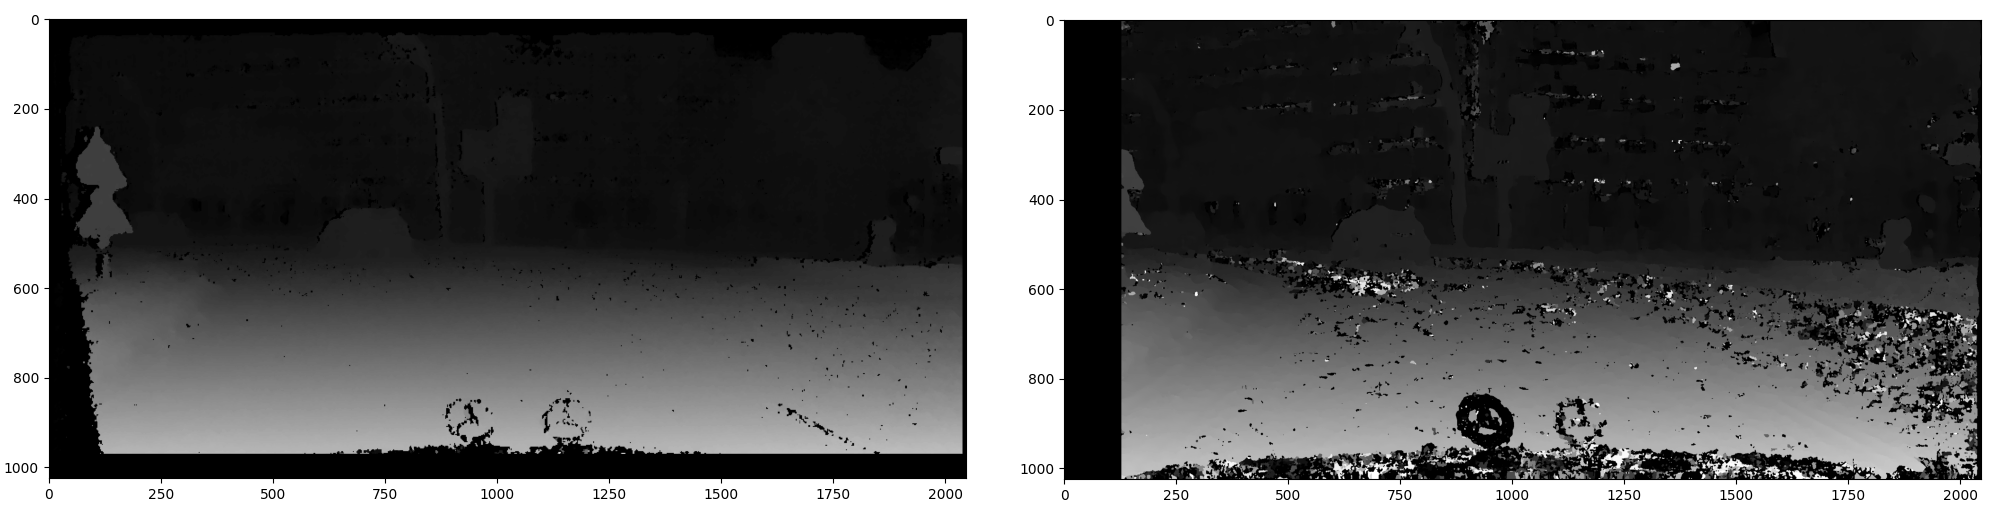
\includegraphics[width=\textwidth]{figures/disparity_1.png}}{disparity example}
\caption[Tämä on lyhyt kuvateksti.]{Vasemmalla tarjottu totuus. Oikealla opencv tulos stereo kuvasta.}
\label{fig:disparity1}
\end{figure}
    
Tästä näemme, että stereokuvasta syvyysdatan kerääminen on mahdollista valmiiksi implimentoiduilla metodeilla opencv2 kirjaston avulla. Blur lisättiin jotta mahdolliset kameran aiheuttamat häiriöt saadaan minimoitua. Käytetyt parametrit tarkoittavat että mahdollisia disparity tasoja on 128 ja alue jolta samankaltaisuutta verrataan on 20 pikselin kokoinen. Functiota ajettin HH modessa, joka tarkoittaa että se suoritetaan algoritmin alkuperäisellä suoritustavalla, eikä kevennetyllä jota käytetään muistin säästämiseksi.

Tuloksestamme huomaamme häiriötä jota totuudessa ei ole. Tämä johtuu todennäköisesti kohdista kuvista joista hismillerin algoritmi ei pysty tunnistamaan vastaavaa kohtaa toisessa kuvassa. Tämä voi tapahtua esimerkiksi asvaltin pinnassa jossa on hyvin samankaltaista tai varjoisilla alueilla. Näistä alueista ei ole niin helppoa löytää uniikkia vertailukohtaa. 

- TODO: "Tätä pitää vielä parannella, näyttää aika ikävältä"

\subsection{Semantic segmentation}

Aineistossa on jo totuus segmentaatio datasta. Käytämme tätä valmiina saatavaa dataa, mutta tämä koulutetaan silti uudelleen. Koulutettu verkko on hyvin yksinkertainen ja käyttää valmiita komponenttejä. Data on koulutettu\ fcn\_resnet50 avulla \cite{pytorchfcnresnet50}, ilman esikoulutettuja painoja cityscapes datasetillä. Optimointiin on käytetty adamia ja loss funktioon CrossEntropyLoss funktiota. Datasetin mallia on yksinkertaistettu tarpeen mukaan. Jolloin kaikki liikkuvat asiat niinkuin autot ja ihmiset ovat yhdessä luokassa ja kaikki muu toisessa. Näin saadaan yksinkertaisempi malli. Näin on saatu lopputulos jonka avulla voidaan nähdä kuvasta kaikki liikkuvat osat \ref{fig:segmentation1}.

\begin{figure}
\centering
\pdftooltip{
\includegraphics[width=\textwidth]{figures/segmentation1.png}}{segmentation example}
\caption[Tämä on lyhyt kuvateksti.]{Vasemmalla tarjottu totuus. Oikealla mallin tuottama.}
\label{fig:segmentation1}
\end{figure}
    

"Tähän pitää lisätä sellainen hieno graafi koulutuksesta niin näyttää hienolta.Selittää miksi adam on valittu ja mikä se on. Selittää miksi crossEntropy on valittu ja mikä se on."

\section{Datasetin muodostus}

- TODO: Kerro eri mahdollisista tavoista datasetin muodostamiseen.

- Vertical ja horistonal swipe. 

- Mahdollisia parempia tapoja jotka vaativat manuaalisempia lähestymistapoja



Kun meillä on syvyysdata ja segmentointi data voimme muodostaa koulutkseen käytettävän mallin. Poistamalla syvyysmuutokset disparity alueilta joissa on liikkuvia asioita, ja olettamalla että niiden takana syvyys muuttuu niinkuin niiden ympärillä voimme muodostaa koulutusdatan jonka avulla voimme yhdestä kuvasta generoida pisteavaruuden ilman liikkuvia asioita.

Tälläinen muodostustapa ei ole täydellinen ja sen tuottamat tulokset pitääkin suureksi osaksi manuaalisesti validoida. Mutta koska validointi voidaan suorittaa hyväksy hyökää tasolla on suuren kuvamäärän läpikäynti hyvin nopeaa.

\section{miten data validoitiin}

- TODO: "Selitys miten käsin sen käyn läpi kun jaksan koodata siihen skriptin"

\section{Lopullinen malli}

- TODO: "Esitellään pari kuvaa mimmosta dataa tuli, kerrotaan mitä mallia käytettiin. Tod näk samaa kuin segmentationissa. Tehdään malli ja ajetaan pari esimerkki kuvaa. Koulutuksen onistuneisuus. Mikä on paras loss functio jne jne."



